\documentclass{beamer}
\usetheme{Boadilla}
\usecolortheme{beaver}

\usepackage[english]{babel}
\usepackage{graphicx}
\usepackage{subcaption}
\usepackage{mathtools}
\usepackage{color}
\usepackage{epstopdf}
\usepackage{booktabs}

\usepackage{makeidx}
\makeindex
\newenvironment{theindex}
 {\let\item\par
  %definitions for subitem etc
  }{}
\newcommand\indexspace{}

\usepackage[nottoc]{tocbibind}
\usepackage[authoryear,round]{natbib}
\bibliographystyle{abbrvnat}

\DeclarePairedDelimiterX{\quality}[1]{\mathcal{F}(}{)}{#1}  % Summarization quality (F)
\DeclarePairedDelimiterX{\coverage}[1]{\mathcal{L}(}{)}{#1}  % Summarization coverage (L)
\DeclarePairedDelimiterX{\diversity}[1]{\mathcal{R}(}{)}{#1}  % Summarization diversity (R)
\newcommand{\budget}{\mathcal{B}}
\newcommand{\sentcost}{c}
\newcommand{\similarity}{\text{M}}  % Individual similarities

\DeclarePairedDelimiterX{\inp}[2]{\langle}{\rangle}{#1, #2}  % Inner product
\definecolor{prettyblue}{HTML}{3333B2}

\title{Event Detection from Text Data}
\author{Tom\'a\v{s} Kala}
\date{June 20, 2017}



\begin{document}

% Introduction
\frame{\titlepage}

% Motivation
\begin{frame}
\frametitle{Event detection}


\begin{itemize}
\item What is it about?
\item Original method by \cite{event-detection}
\item Our contribution (through Word2Vec)
\end{itemize}

\begin{figure}

\centering
\includegraphics[width=\linewidth,height=\textheight,keepaspectratio]{charlie_hebdo}
\caption{6/1 - 17/1, 2015: V redakci satirick\'eho listu Charlie Hebdo v Pa\v{r}\'i\v{z}i se st\v{r}\'ilelo. Francouzsk\'y satirick\'y \v{c}asopis Charlie Hebdo, na kter\'y minul\'y t\'yden za\'uto\v{c}ili islamist\'e, znovu vyd\'a karikatury proroka Mohameda.}
\end{figure}


\end{frame}

% Word2Vec
\begin{frame}
\frametitle{Word2Vec}

\begin{itemize}
\item Neural network language model by \cite{word2vec}
\item Learns vector representation that preserves word properties
\end{itemize}

\begin{columns}
\begin{column}{0.5\textwidth}
\centering
\begin{figure}
\includegraphics[width=\linewidth,height=0.5\textheight,keepaspectratio]{word2vec_diagrams}
\caption{Word2Vec schema}
\end{figure}
\end{column}

\begin{column}{0.5\textwidth}
\begin{table}
\begin{tabular}{ c | c}\toprule[1.5pt]
\bf terorista & \bf olympi\'ada \\ \midrule
islamista & olympijsk\'y \\
d\v{z}ih\'adista & paralympi\'ada \\
extremista & univerzi\'ada \\
teroristick\'y & So\v{c}a \\
Coulibaly & medailista \\
allah & So\v{c}i \\
ozbrojenec & v\'iceboj \\
d\v{z}ih\'ad & mistrovstv\'i \\
isl\'amsk\'y & \v{s}ampion\'at \\ \bottomrule[1.25pt]

\end{tabular}
\caption{Most similar words}
\end{table}
\end{column}
\end{columns}

\end{frame}

% Word representation
\begin{frame}
\frametitle{Word representation}
\framesubtitle{Each word abstracted into 2 vectors}

\begin{enumerate}
\item Semantical representation -- vector space embedding

\begin{equation}
\mathbf{v}_{w} \in \mathbb{R}^{100}\ \text{(learned through Word2Vec).}
\end{equation}

\item Trajectory -- Document Frequency-Inverse Document Frequency

\begin{equation}
\mathbf{y}_{w} \in \mathbb{R}^{T},~\mathbf{y}_{w}(t) = \underbrace{\frac{\text{DF}_{w}(t)}{\text{N}(t)}}_{\text{DF}} \cdot \underbrace{\log{\frac{N}{\text{DF}_{w}}}}_{\text{IDF}},\ t = 1, \dots, T
\end{equation}

\end{enumerate}

\end{frame}

% Word trajectories examples
\begin{frame}
\frametitle{Word trajectories}

\begin{figure}
        \centering
        \begin{minipage}{.5\textwidth}
            \centering
            \includegraphics[width=\linewidth]{christmas}
            \caption{An important word (Christmas)}
        \end{minipage}%
        \begin{minipage}{.5\textwidth}
            \centering
            \includegraphics[width=\linewidth]{friday}
            \caption{A stopword (Friday)}
        \end{minipage}
    \end{figure}

Signal power decides between the two categories.
\end{frame}

% Event detection 1
\begin{frame}
\frametitle{Event detection}
\framesubtitle{Original method and its modification}

\begin{columns}

\begin{column}{0.45\textwidth}
\begin{enumerate}

\item Original greedy optimization:
\begin{itemize}
\item KL-divergence of the trajectories
\item Simple document overlap
\item 217 events, 2.08 keywords/event
\item Too strict
\end{itemize}

\item Word2Vec-based modification:
\begin{itemize}
\item Cosine similarity of word vectors
\item 46 events, 10.28 keywords/event
\item Too noisy
\end{itemize}

\end{enumerate}
\end{column}

\begin{column}{0.55\textwidth}
\begin{figure}
\centering
\includegraphics[width=\linewidth,height=\textheight,keepaspectratio]{charlie_hebdo_sucky_quality}
\end{figure}

\begin{figure}
\centering
\includegraphics[width=\linewidth,height=\textheight,keepaspectratio]{greedy_sucks}
\end{figure}
\end{column}

\end{columns}

\end{frame}

% Event detection 2
\begin{frame}
\frametitle{Event detection}
\framesubtitle{Cluster-based algorithm}

\begin{itemize}
\item Application of DBSCAN \citep{dbscan}
\item Custom distance function
\item Trajectory filtering
\item 77 events, 9.88 keywords/event
\end{itemize}

\begin{figure}
\centering
\includegraphics[width=\linewidth,height=\textheight,keepaspectratio]{ebola}
\end{figure}
\end{frame}

% Document retrieval
\begin{frame}
\frametitle{Document retrieval}
\begin{minipage}[c]{0.50\textwidth}
\begin{itemize}
\item Event trajectories
\item Active periods
\item Keywords as a query
\end{itemize}
\end{minipage}
\hfill
\begin{minipage}[c]{0.45\textwidth}
\begin{figure}
\centering
   \begin{subfigure}{\textwidth}
   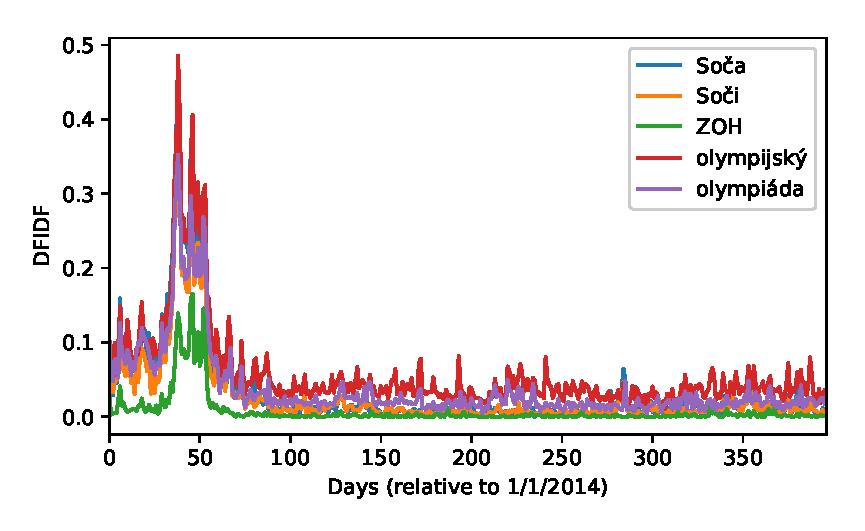
\includegraphics[width=1\linewidth]{39_words}
\end{subfigure}

\begin{subfigure}{\textwidth}
   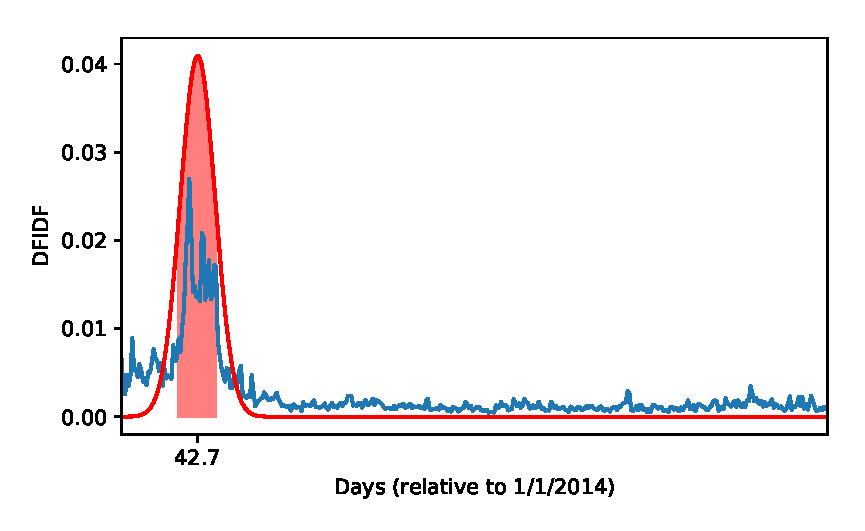
\includegraphics[width=1\linewidth]{39_density_fit}
   \caption*{{\color{prettyblue}Figure:} Gaussian fit, active period = $[\mu - \sigma, \mu + \sigma]$}
\end{subfigure}
\end{figure}
\end{minipage}
\end{frame}

% Annotation
\begin{frame}
\frametitle{Event annotation}
\begin{block}{Document headlines not informative enough}
Charlie Hebdo op\v{e}t otiskne karikatury proroka Mohameda
\end{block}
Multi-document summarization \citep{multi-summarization-1, multi-summarization-2}
\begin{equation}
\begin{alignedat}{-1}
\max_{S \subseteq U} & \quad \quality{S} = \coverage{S} + \lambda \diversity{S} \\
\text{s. t.} & \quad \sum_{i \in S}{\sentcost_{i}} \leq \budget
\end{alignedat}
\end{equation}

\begin{block}{We ran into some issues...}
\dots Pak ale za\v{c}alo zab\'ijen\'i v centru Pa\v{r}\'i\v{z}e. \dots \ Sloni v zoo Dv\r{u}r Kr\'alov\'e si pochutnali na vano\v{c}n\'ich stromc\'ich. \dots
\end{block}

\end{frame}

% Results
\begin{frame}
\frametitle{Results}
\centering
\resizebox{\columnwidth}{!}{%
\begin{tabular}{ l c c c | c | c | c}\toprule[1.5pt]
\bf Method 	 & \bf P & \bf R & \bf $\mathbf{F_{1}}$ & \bf Redundancy & \bf Noisiness & \bf Purity \\ \midrule
\bf Original &  16.35\%     & \bf 28.57\%     &  20.80\% & 77.99\% & 50.94\% & 30.53\% \\
\bf Modified   &  8.70\%     & 10.20\%      &  9.39\% & 65.22\% & 19.57\% & 44.42\% \\
\bf Clusters &  \bf 25.97\%     & \bf 28.57\%      & \bf 27.21\% & \bf 42.86\% & \bf 19.48\% & \bf 61.08\%\\ \bottomrule[1.25pt]
\end {tabular}%
}\par
\captionof{table}{Precision, Recall, Redundancy, Noisiness and Purity comparison} \label{tab:title}

\par

\centering
\begin{tabular}{ r c c c }\toprule[1.5pt]
\bf Unit & \bf Original & \bf Modified & \bf Clusters \\ \midrule
Word2Vec & N/A & \multicolumn{2}{c}{3h 50min} \\
Word analysis & $\longleftarrow$ & 37min & $\longrightarrow$ \\
Event detection & 2min 12s & 38s & 4min 50s \\
Document retrieval & 7min 30s & 6h & 7h 40min \\
Event annotation & 3h 22min & 3min 38s & 7min 30s \\ \midrule
\bf Total & 4h 9min & 10h 31min & 12h 20min\\ \bottomrule[1.25pt]

\end{tabular}\par
\captionof{table}{Computation time comparison} \label{tab:title}
\end{frame}

% Conclusion
\begin{frame}
\frametitle{Conclusion, use case}

\begin{itemize}
\item Event detection with low redundancy
\item Subsequent document retrieval
\item Human-readable annotations
\end{itemize}

\begin{figure}
\centering
\includegraphics[width=\linewidth,height=\textheight,keepaspectratio]{crime_events_highlighted_trajectories}
\end{figure}

\begin{figure}
\centering
\includegraphics[width=\linewidth,height=\textheight,keepaspectratio]{crime_events_highlighted_averaged}
\end{figure}
\end{frame}


% Bibliography
\begin{frame}[shrink=20,noframenumbering]
\frametitle{Bibliography}
\bibliography{sources}
\end{frame}


% Word representation full
\begin{frame}[noframenumbering]
\frametitle{Word representation}
\framesubtitle{Each word abstracted into 2 vectors}

\begin{enumerate}
\item Semantical representation -- vector space embedding

\begin{equation}
\mathbf{v}_{w} \in \mathbb{R}^{100}\ \text{(learned through Word2Vec).}
\end{equation}

\item Trajectory -- Document Frequency-Inverse Document Frequency

\begin{equation}
\mathbf{y}_{w} \in \mathbb{R}^{T},~\mathbf{y}_{w}(t) = \underbrace{\frac{\text{DF}_{w}(t)}{\text{N}(t)}}_{\text{DF}} \cdot \underbrace{\log{\frac{N}{\text{DF}_{w}}}}_{\text{IDF}},\ t = 1, \dots, T
\end{equation}

with

\begin{itemize}
\item T \dots~document stream length (in days),
\item N \dots~number of documents,
\item $\text{N}(t)$ \dots~\# of documents published on day $t$,
\item $\text{DF}_{w}$ \dots~\# of documents containing the word $w$,
\item $\text{DF}_{w}(t)$ \dots~\# of documents containing the word $w$ published on day $t$.
\end{itemize}

\end{enumerate}

\end{frame}


% Annotation full
\begin{frame}[noframenumbering]
\frametitle{Multi-document summarization}
\begin{equation}
\begin{alignedat}{-1}
\max_{S \subseteq U} & \quad \quality{S} = \coverage{S} + \lambda \diversity{S} \\
\text{s. t.} & \quad \sum_{i \in S}{\sentcost_{i}} \leq \budget,~\text{with}
\end{alignedat}
\end{equation}

\begin{itemize}
\item U \dots~set of all sentences,
\item $\mathcal{L}$ \dots~relevance measure composed of sentence pairwise similarities,
\item $\mathcal{R}$ \dots~diversity measure controlled by $\lambda$,
\item $\mathcal{B}$ \dots~maximum summary length,
\item $c_{i}$ \dots~length of sentence $i$.
\end{itemize}

\end{frame}


% WMD
\begin{frame}[noframenumbering]
\frametitle{Word Mover's Distance}
\begin{itemize}
\item Document similarity measure by \cite{wmd}
\item Transportation problem between word vectors of 2 documents
\end{itemize}

\begin{columns}
\begin{column}{0.55\textwidth}
\small
\begin{equation}
\begin{alignedat}{-1}
\min_{\mathbf{T} \geq 0} & \quad \sum_{i,j = 1}^{n} \mathbf{T}_{ij} \| \mathbf{x}_{i} - \mathbf{x}_{j} \|_{2} \\
\text{s. t.} & \quad \sum_{j=1}^{n} \mathbf{T}_{ij} = d_{i} \quad \forall i \in \{1, \dots, n \} \\
& \quad \sum_{i=1}^{n} \mathbf{T}_{ij} = d'_{j} \quad \forall j \in \{1, \dots, n \}
\end{alignedat}
\end{equation}
\normalsize
\end{column}

\begin{column}{0.45\textwidth}
\begin{itemize}
\item $n$ \dots vocabulary size
\item $\mathbf{x}_{i}$ \dots vector embedding of the word $i$
\item $d_{i}$ ($d'_{i}$) \dots normalized frequency of $i$ in document 1 (2)
\end{itemize}
\end{column}
\end{columns}

\begin{figure}
\centering
\includegraphics[height=0.2\textheight]{wmd_flow}
\caption{WMD illustration}
\end{figure}

\end{frame}



\end{document}
